%!TEX root = ../master.tex
\chapter{Code Overview}\label{ch:codeover}

The structure of the implemented software can be seen in the class diagram in Figure~\ref{fig:implementedClassDiagram}.

\begin{figure}
	\centering
	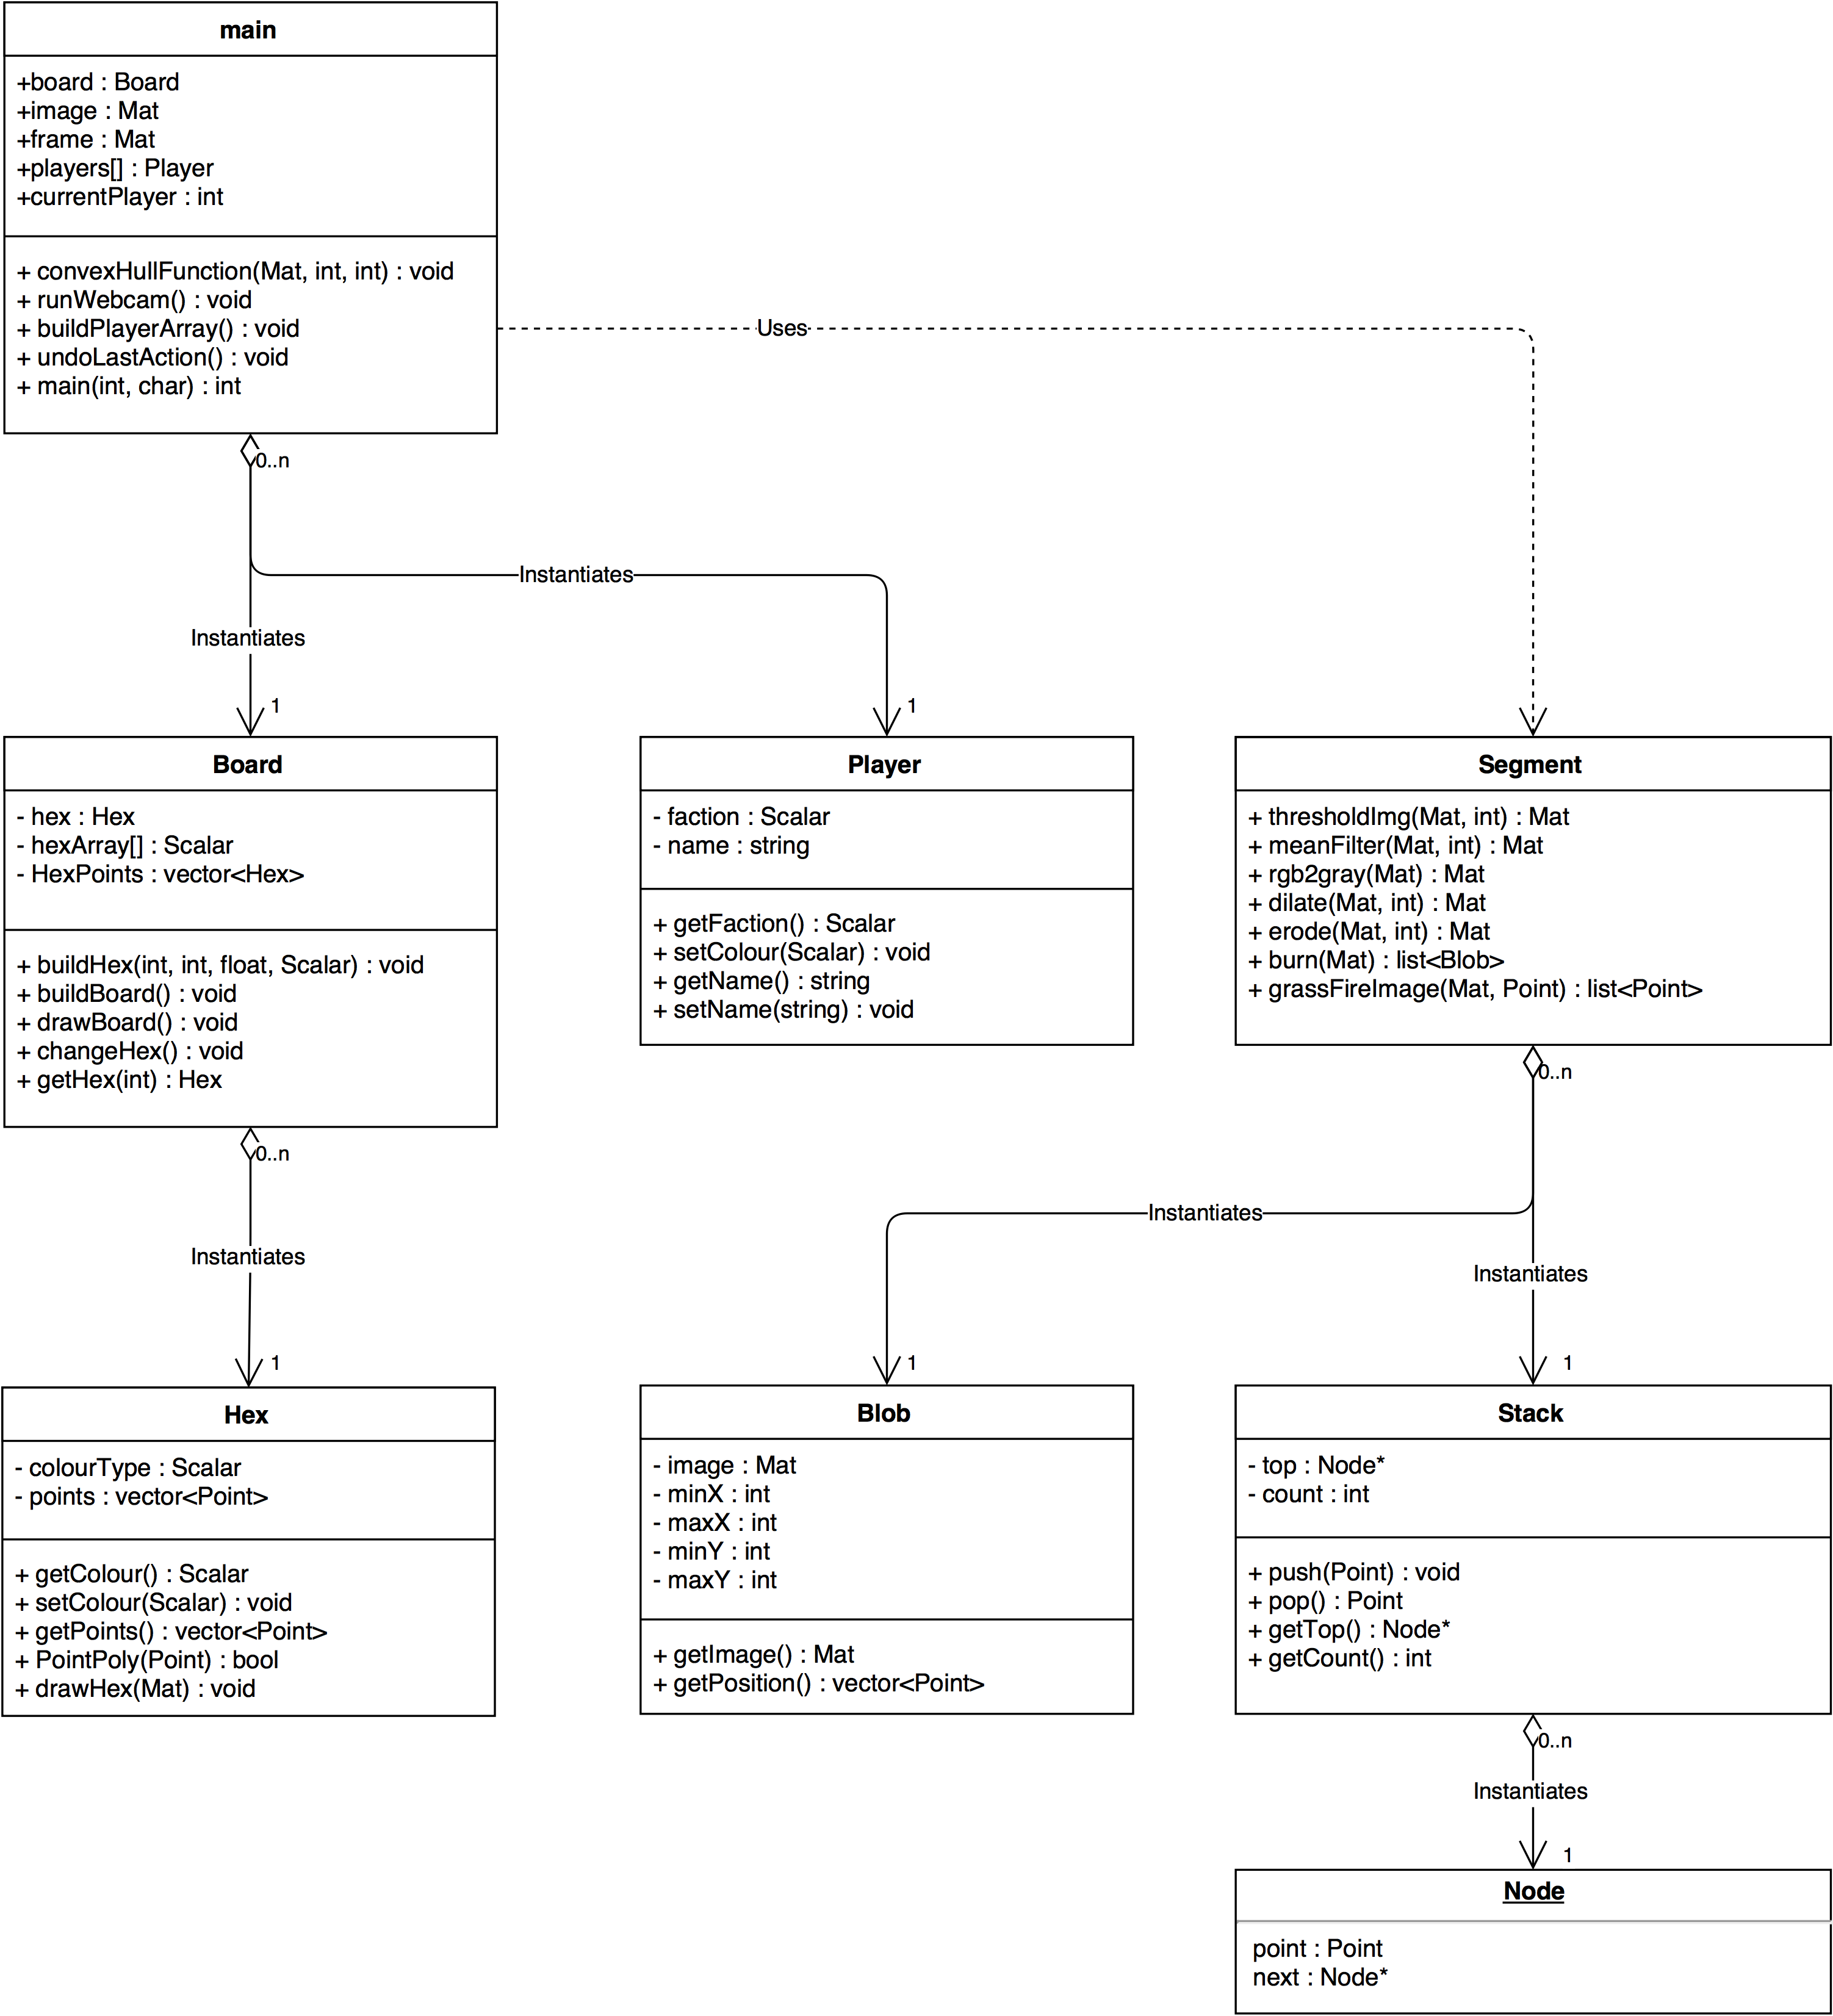
\includegraphics[width=1\textwidth]{ImplementedClassDiagram}
	\caption{Class diagram of the software \label{fig:implementedClassDiagram}}
	
\end{figure}

\section{Segment namespace}
\texttt{Segment} is a namespace which includes all image processing algorithms used in the software which are not standard OpenCV methods.

\subsection{Point-processing}
There are three point-processing algorithms in this software; an RGB-to-Greyscale colour conversion algorithm, a normalization algorithm, and a thresholding algorithm. All of these make use of double-nested \texttt{for}-loops to apply their operations to each pixel as shown in Figure~\ref{fig:pointprocess}.
\begin{figure}[!h]
\begin{lstlisting}
for (int y = 0; y < src.rows; ++y)
{
	for (int x = 0; x < src.cols; ++x)
	{
		//Code here...
	}
}
\end{lstlisting}
\caption{Basic point-processing algorithm. \label{fig:pointprocess}}
\end{figure} 

The RGB-to-Greyscale algorithm creates an 8-bit single-channel image and then maps the mean of the RGB-values of the input image pixels to the output like shown in Figure~\ref{fig:rgb2gray}

\begin{figure}[!h]
\begin{lstlisting}
output.at<uchar>(y, x) = (src.at<Vec3b>(y, x)[0] + src.at<Vec3b>(y, x)[1] + src.at<Vec3b>(y, x)[2]) / 3;
\end{lstlisting}
\caption{RGB-to-Greyscale operation.\label{fig:rgb2gray}}
\end{figure}

The normalization algorithm finds the maximum and minimum pixel values of the input image using an OpenCV function. It then processes each pixel to normalize them to a new maximum and minimum using the operation shown in Figure~\ref{fig:normalize}.

\begin{figure}
\begin{lstlisting}
output.at<uchar>(y, x) = floor((src.at<uchar>(y, x) - min) * (newMax - newMin) / (max - min) + newMin);
\end{lstlisting}
\caption{Normalization of a pixel. \label{fig:normalize}}
\end{figure} 

Finally, the thresholding algorithm determines whether a given output pixel is white or black based on the if-else statement that is shown in Figure~\ref{fig:threshold}.

\begin{figure}
\begin{lstlisting}
if (src.at<uchar>(y, x) >= threshold)
{
	src.at<uchar>(y, x) = 255;
}
else
{
	src.at<uchar>(y, x) = 0;
}
\end{lstlisting}
\caption{Thresholding. If the pixel value is above the threshold, make it white. Else, make it black.\label{fig:threshold}}
\end{figure}

\subsection{Neighbourhood processing}
The neighbourhood processing methods used in this software are \texttt{erode}, \texttt{dilate} and \texttt{gaussianFilter}. These filters apply their kernels to each pixel through the process of convolution. That is to say, for each pixel they calculate a value for each pixel relative to the processed pixel based on the kernel. These results are then used for further calculations depending on the purpose of the filter.

The filters make use of a nested \texttt{for}-loop similar to the point-processing algorithms to go through each pixel. This loop can be seen in Figure~\ref{fig:neighbourhoodForLoop}. The main difference in this loop from the point-processing loop is, that this one ignores pixels at the edge of the image. This is to avoid \textit{out of bound} errors, since reading a pixel value outside an image makes OpenCV throw an exception.

\begin{figure}
\begin{lstlisting}
for (int y = 0 + kernRad; y < src.rows - kernRad; ++y)
{
	for (int x = 0 + kernRad; x < src.cols - kernRad; ++x)
	{
		//Code here...
	}
}
\end{lstlisting}
\caption{Neighbourhood processing loop that reads each pixel in an image except those at the edge. \label{fig:neighbourhoodForLoop}}
\end{figure}

\texttt{erode} and \texttt{dilate} are essentially inversions of each other. They take binary images as arguments. \texttt{dilate} is what is known as a \texttt{hit} algorithm. It checks whether any pixel within the kernel is white (has a value of 255). If that is the case, the processed pixel is made white, otherwise it is made black. This can be seen in Figure~\ref{fig:dilateAlgorith}. \texttt{erode}, by contrast is a \textit{fit} algorithm. Like \texttt{dilate} it checks whether any pixel within the kernel is white. If any of the pixels in the kernel are not white, the pixel is made black. Only if all of the pixels are white will the processed pixel be white. This can be seen in Figure~\ref{fig:erodeAlgorithm}.

\begin{figure}
\begin{lstlisting}
for (int ky = y - kernRad; ky <= y + kernRad; ++ky)
{
	for (int kx = x - kernRad; kx <= x + kernRad; ++kx)
	{
		if (src.at<uchar>(ky, kx) == 255) {
			Temp++;
		}
	}
}
//if one of the pixels are value 255, give the output pixel greyscale value of 255
if (Temp != 0){
	output.at<uchar>(y, x) = 255;
}
//else, give it 0
else {
	output.at<uchar>(y, x) = 0;
}
Temp = 0;
\end{lstlisting}
\caption{The dilation algorithm \label{fig:dilateAlgorith}}
\end{figure}

\begin{figure}
\begin{lstlisting}
for (int ky = y - kernRad; ky <= y + kernRad; ++ky)
{
	for (int kx = x - kernRad; kx <= x + kernRad; ++kx)
	{
		if (src.at<uchar>(ky, kx) == 255) {
			Temp++;
		}
	}
}
//if all the pixels are value 255, give the output pixel greyscale value of 255
if (Temp == kernPixels){
	output.at<uchar>(y, x) = 255;
}
//else, give it 0
else {
	output.at<uchar>(y, x) = 0;
}
Temp = 0;
\end{lstlisting}
\caption{The erotion algorith\label{fig:erodeAlgorithm}}
\end{figure}

\section{BLOB extraction}
After segmentation, a grass-fire implementation scans the image for BLOBs. First, a nested \texttt{for}-loop like the one shown in Figure~\ref{fig:pointprocess} goes through every pixel to check whether any of them is white (i.e. part of the foreground). If this condition is met, the function will call another function, which contains the actual grass-fire algorithm. The grass-fire function is called with the position of the white pixel and the image itself as arguments. 

\section{Board class}
The rendered board consists of a hexagonal grid placed on top of a pre-made image.  Initially, the \texttt{buildBoard()} method in the \texttt{Board} class is called. This method assigns a Scalar value to each position in an array each of which correspond to a hexagon on the board. This assignment of colours is hard-coded since the layout is static with no apparent pattern to dynamically generate the hexagons from. Then, the position of each of the hexagons is calculated.